
\chapter{Разработка программы решения теоретико-графовой задачи на
  языке программирования C++ с использованием семантической памяти}
\label{cha:libscalgo}

Для понимания этой главы студент должен обладать следующими знаниями:

\begin{itemize}
\item базовыми знаниями по языку C++
\item базовыми знаниями по работе с STL-контейнерами
  \lstinline|std::set|, \lstinline|std::map|, \lstinline|std::list|,
  \lstinline|std::pair|
\end{itemize}

\section{Задание}
\label{sec:libscalgo_task}

На этом этапе выполнения расчетной работы вам необходимо будет
разработать программу с использованием библиотеки моделирования
sc-памяти, которая бы решала вашу теоретико-графовую задачу на основе
формализации предметной области, проведенной на предыдущем этапе
(см. главу~\ref{cha:onto}). Сам алгоритм вы уже исследовали в прошлом
семестре (см. главы~\ref{cha:cppalgo}~и~\ref{cha:algodemo}), но сейчас
надо будет не просто реализовать какой-то алгоритм, а адаптировать его
к графодинамическому способу обработки информации. Это значит, что вся
информация, необходимая для работы вашего алгоритма, должна храниться
в sc-памяти и там же обрабатываться. В качестве примера
<<неудобства>>, которое вам может принести такое требование, я могу
привести невозможность использования привычной матрицы
смежности/инцидентности.  Поэтому для прохождения этого этапа вам
придется взглянуть на алгоритм, решающий выбранную задачу, под другим
углом.

В качестве тестов для написанной программы необходимо использовать
тестовые примеры, которые вы сделали в ходе предыдущих этапов
расчетной работы.

\section{Установка и настройка рабочей среды}
\label{sec:libscalgo_setup}

Для начала мы установим и настроим рабочую среду для программирования
с использованием программной модели sc-памяти и запустим
программу-пример, которая использует эту библиотеку.

Во-первых, нам необходимо скачать и установить программный модуль
\texttt{sc-core}, который представляет собой ядро для обработки
sc-текстов:

\begin{itemize}
\item \verb|sc-core-0.2.5-win32.exe| работает с \texttt{MS Visual Studio 9}
\item \verb|sc-core-0.2.5-vc10-bin-win32.exe| работает с \texttt{MS Visual Studio 10}
\end{itemize}

После того, как вы скачали инсталлятор, запустите его. Желательно
устанавливать \texttt{sc-core} так, чтобы полный путь к установленной
папке не содержал пробелов в именах директорий. При установке
необходимо выбрать опцию, которая добавит директорию исполняемых
файлов \texttt{sc-core} в переменную среды окружения \verb|PATH|
(см. рис.~\ref{fig:Add_sc_core_to_path}).

\begin{figure}[h!]
  \centering
  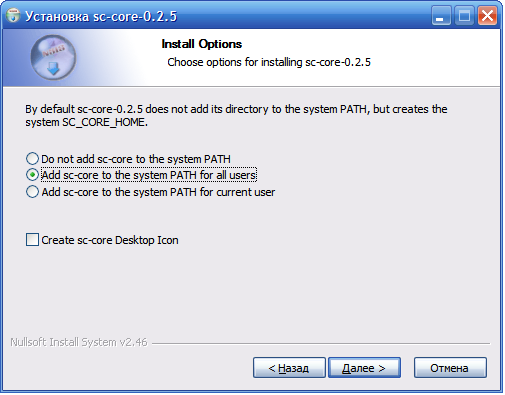
\includegraphics[scale=0.7]{4/setup/Add_sc_core_to_path}
  \caption{Добавление директории исполняемых файлов \texttt{sc-core} в
    системную переменную \texttt{PATH} для всех пользователей}
  \label{fig:Add_sc_core_to_path}
\end{figure}
 
Мной была выбрана установка \texttt{sc-core} в папку
\verb|c:\sc-core|. После установки данного модуля были изменены
следующие переменные среды окружения:

\begin{itemize}
\item \verb|SC_CORE_HOME|, которая теперь имеет значение
  \verb|c:\sc-core|
\item \verb|PATH|, к которой была добавлена директория
  \verb|c:\sc-core\bin|
\end{itemize}

В дальнейшем для указания пути к директории \texttt{sc-core} я буду
использовать значение переменной среды окружения \verb|SC_CORE_HOME|.

Для сборки примера нам еще будет необходима программа
\texttt{\href{http://www.cmake.org/}{CMake}}. Необходимо скачать
установочный файл для версии не ниже \texttt{2.6.2}. Как и при
установке \texttt{sc-core}, при установке \texttt{CMake} необходимо
выбрать опцию, которая добавит директорию исполняемых файлов в
переменную среды окружения \verb|PATH|
(см. рис.~\ref{Add_cmake_to_path}).
 
\begin{figure}[h]
  \centering
  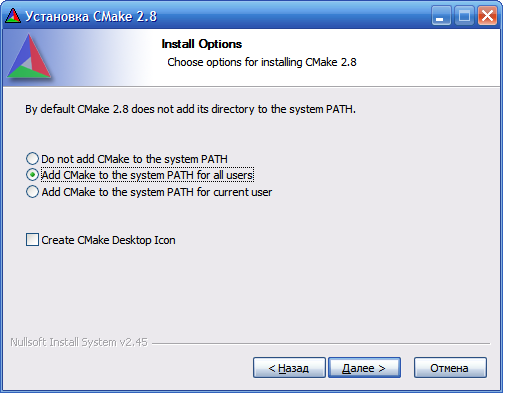
\includegraphics[scale=0.7]{4/setup/Add_cmake_to_path}
  \caption{Добавление \texttt{CMake} в системную переменную
    \texttt{PATH} для всех пользователей}
  \label{fig:Add_cmake_to_path}
\end{figure}

С модулем \texttt{sc-core} версии \texttt{0.2.5} идет старая версия
примера использования библиотеки моделирования sc-памяти, поэтому
необходимо с сервера \texttt{Info} взять новую версию примера
\verb|wave_find_path|. Для этого необходимо скопировать всю папку \verb|wave_find_path| в:

\begin{verbatim}
%SC_CORE_HOME%\examples\wave_find_path
\end{verbatim}

Для генерации проекта примера воспользуемся консолью. Для запуска
консоли нажимаем клавиши \verb|Win + R|, в появившемся диалоге пишем
\verb|cmd| и нажимаем \texttt{Enter}. На экране должно появиться окно,
как показано на рис.~\ref{fig:Run_console}.

\begin{figure}[h!]
  \centering
  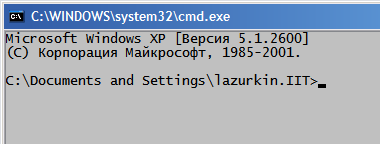
\includegraphics[scale=0.7]{4/setup/Run_console}
  \caption{Открытая консоль}
  \label{fig:Run_console}
\end{figure}

Переходим в директорию примера, используя команды:

\begin{verbatim}
c: 
cd %SC_CORE_HOME%\examples\wave_find_path
\end{verbatim}

\begin{figure}[h]
 \centering
 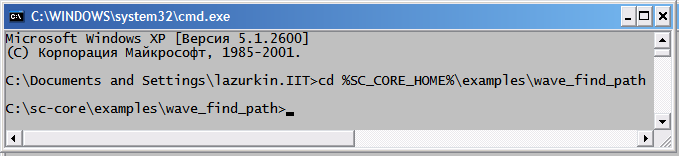
\includegraphics[scale=0.7]{4/setup/Cd_to_example_dir}
 \caption{Переход в директорию примера \texttt{wave\_find\_path}}
  \label{fig:cd_to_example_dir}
\end{figure}

Если у вас Windows с русификацией, то могут возникнуть проблемы с
запуском \texttt{cmake}. \texttt{CMake} будет сообщать о том, что он
не может скопировать файлы \verb|CMakeVSMacros1.vsmacros| и
\verb|CMakeVSMacros2.vsmacros| в (это путь на моей файловой системе с
моим именем пользователя, для вас он будет отличаться названием
директории вашего пользователя):

{\footnotesize
\begin{verbatim}
c:\Documents and Settings\lazurkin.IIT\Мои документы\Visual Studio 2008\Projects\VSMacros80\CMakeMacros
\end{verbatim}
}

Эти файлы необходимо скопировать вручную. Для этого просто скопируйте
содержимое

{\footnotesize
\begin{verbatim}
c:\Program Files\cmake2.8\share\cmake-2.8\Templates\
\end{verbatim}
}

в

{\footnotesize
\begin{verbatim}
c:\Documents and Settings\lazurkin.IIT\Мои документы\Visual Studio 2008\Projects\VSMacros80\CMakeMacros
\end{verbatim}
}

При помощи следующей команды сгенерируем проект \texttt{MS Visual
  Studio 9.0} для сборки и запуска примера (в \texttt{cmake} есть
генератор и для \texttt{MS Visual Studio 10.0}, просто введите команду
\texttt{cmake} и на консоль будет выведен список всех доступных
генераторов):

\begin{verbatim}
cmake -G "Visual Studio 9 2008" .
\end{verbatim}

\begin{figure}[h!]
  \centering
  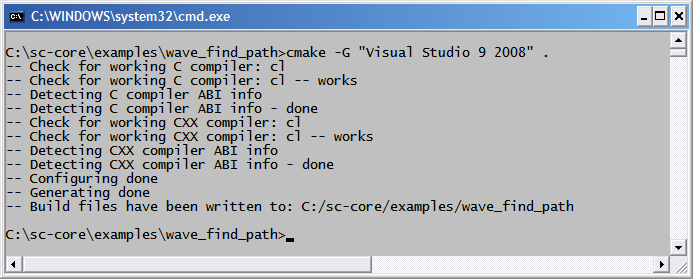
\includegraphics[scale=0.7]{4/setup/Generate_project}
  \caption{Генерация проекта для примера \texttt{wave\_find\_path}}
  \label{fig:gen_project}
\end{figure}

Если у вас \texttt{MS Visual Studio 2010}, то можете попробовать
команду:

\begin{verbatim}
cmake .
\end{verbatim}

После корректной работы \texttt{CMake} в директории будет создан
проект \verb|wave_find_path|. Открываем его при помощи \texttt{MS
  Visual Studio 9.0}. Нажимаем правой кнопкой мыши на проекте
\verb|wave_find_path| в \texttt{Solution Explorer} и выбираем пункт
меню \texttt{"Set as StartUp Project"}. После этого название данного
проекта будет выделено жирным цветом. Теперь можно запустить на
исполнение пример \verb|wave_find_path| (пример вывода на
рис.~\ref{fig:run_example}).

\begin{figure}[h!]
  \centering
  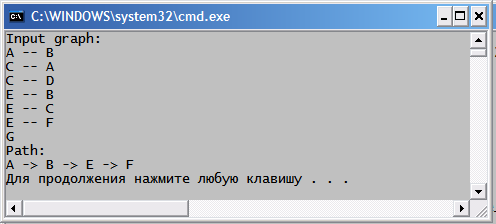
\includegraphics[scale=0.7]{4/setup/Run_example}
  \caption{Вывод работы программы-примера \texttt{wave\_find\_path}}
  \label{fig:run_example}
\end{figure}

%%% Local Variables: 
%%% mode: latex
%%% TeX-master: "ai_rr"
%%% End: 
